
\section{Temporal Analysis}
\label{sec:temporal}

This section presents our study of the temporal property of VirusTotal malwares. 

\begin{figure}[t!]
\begin{center}
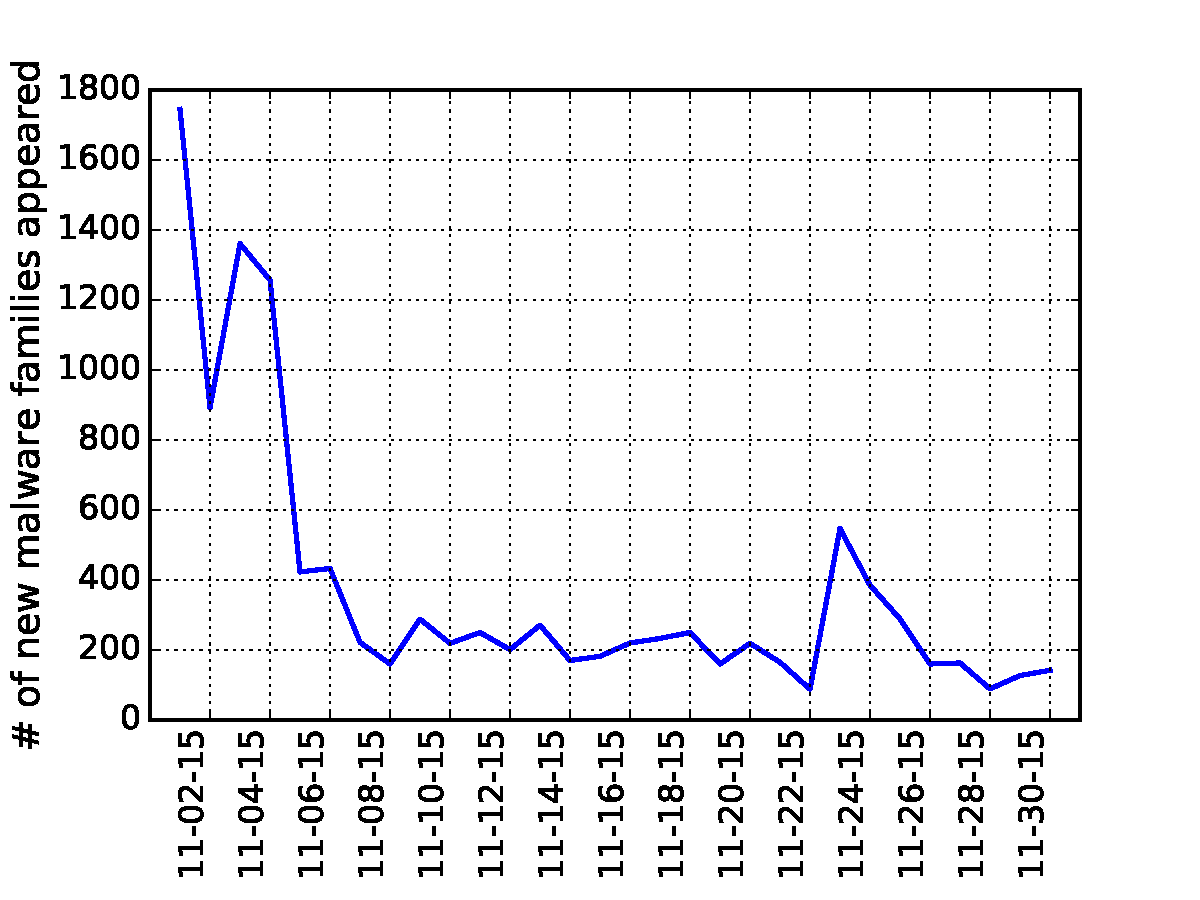
\includegraphics[width=2.5in]{figure/new_family}
\mycaption{fig:new}{New malware families on VirusTotal in November 2015.}
{The number of new malware families we observed every day in November 2015.}
%\label{fig:new}
\end{center}
\vspace{-0.3in}
\end{figure}


We first study how many new malware families appear everyday. 
Figure~\ref{fig:new} shows the number of new malware families appearing on each day in November 2015. 
Since we do not include data before November 1, 
there are more new malware families in the first few days.
After that, the number of new malware families becomes stable, 
falling into a range between 100 and 400. 
In total, there are 11311 malware families in this time period. 

{\bf Observation 1:} 
{\em 100-400 new malware families appear each day.}

\begin{figure}[t!]
\begin{center}
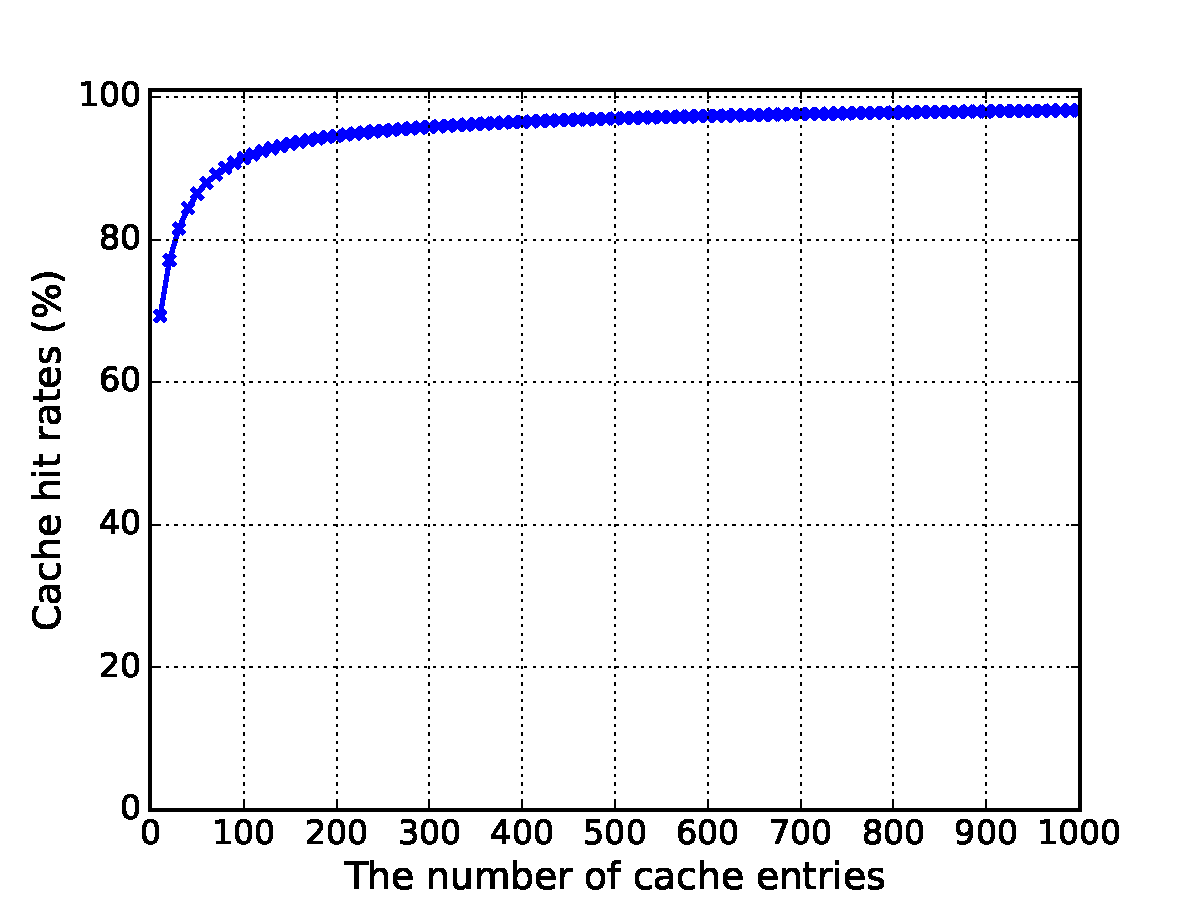
\includegraphics[width=2.5in]{figure/LRU}
\mycaption{fig:cache}{Relation between cache hit rate and cache size.}
{How cache hit rate changes with the change of cache size from 10 to 1000.}
%\label{fig:cache}
\end{center}
\end{figure}
\begin{figure}[t!]
\begin{center}
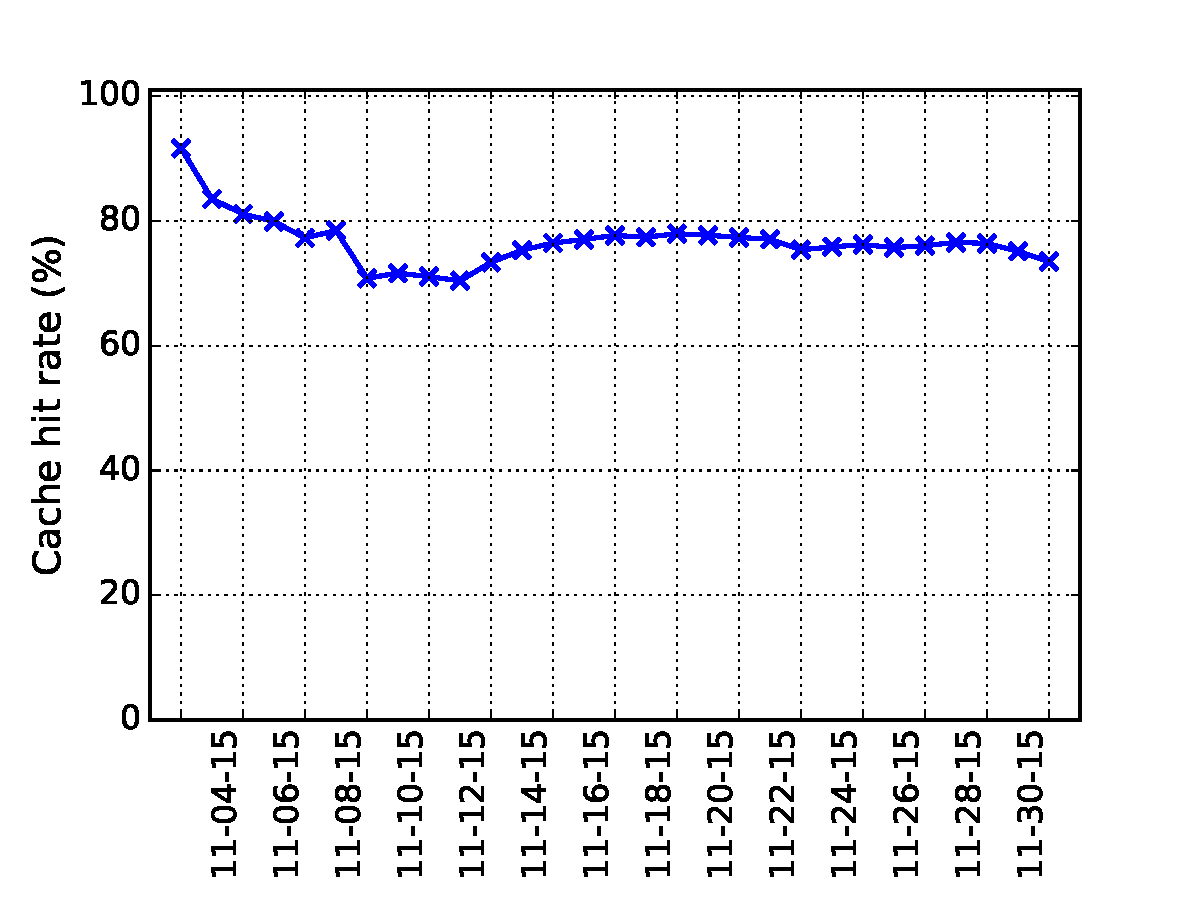
\includegraphics[width=2.5in]{figure/LRU_day}
\mycaption{fig:batchcache}{Cache hit rate in November 2015.}
{Cache hit rate every day in November 2015 if we only update cache content at the end of every day.}
%\label{fig:batchcache}
\end{center}
\vspace{-0.1in}
\end{figure}


Next, we investigate whether malwares behave temporal locality.
Temporal locality is an important metric that can guide the 
prediction of near-future malwares.

Specifically, we analyze how bursty malwares in the same family appear.  
Inspired by previous usage of cache mechanisms in predicting bugs~\cite{predicting},
we design a new cache mechanism to study the burstiness of malwares.

We view malware submission reports as a stream of inputs 
and feed the stream into a cache. 
Each input (\ie, each report) is associated with an address (the family it belongs to) and a time (the submission time of the file).
Thus, a cache hit means that the new report belongs to a family that is currently in the cache,
\ie, the new input has the same address as an entry in the cache.
Therefore, a high cache hit rate implies that the occurance of malwares exhibit temporal locality.

As with general cache mechanisms such as CPU caches and file system buffer caches, 
there are several parameters to tune in a cache.
The cache block size, or cache line size, controls the granularity of cache management, 
\ie, how many entries are inserted into and evicted from cache together.
Cache prefetching loads spacially close entries into caches in advance. 
Cache replacement policy controls what entries to evict when cache is full.
We use a simple cache setting in our evaluation. 
We fix the cache block size to be one, no prefetching, 
and use the LRU (least recently used) replacement policy.

Our malware family cache works as follows.
We start with an empty cache. 
For a new file submission, if the malware family is already in the cache, 
we move the hit cache entry to the front of our cache entry list. 
If the new malware family is not in the cache, 
we create a new cache entry and add it into the front of the cache entry list.
If the cache is full, we evict the entry at the end of the list. 
The cache hit rate is calculated as follows: 

$$ \mbox{hit rate} = \dfrac{\mbox{\# of hits}}{\mbox{\# of hits + \# of misses}}$$

We implemented this malware family cache using Python
and conducted experiments on an AWS c4.4xlarge virtual machine, 
which contains 16 virtual cpus and 30\,GB memory.

We conducted two experiments. 
The first experiment explores how the cache hit rate changes with the number of cache entries. 
We change the cache size from 10 to 1000. 
As shown in Figure~\ref{fig:cache}, the hit rate grows from 69.29\% to 98.14\%. 
When using more than 80 cache entries, which is less than 1\% of the total number of malware families, the cache hit rate rises above 90\%, 
and when using more than 230 cache entries, which is less than 3\% of the total number of malware families, 
the cache hit rate rises above 95\%. 
The high cache hit rate confirms that malwares occur in bursts.

In the second experiment, we fix the cache size to 100 
and lower the cache content update frequency from once per malware report to once per day.
That is, we keep cache content unchanged to count cache hits and cache misses each day and update the cache content at the end of each day.
Figure~\ref{fig:batchcache} shows the cache hit rate for each day. 
Most cache hit rate falls in a range between 70\% and 80\%.  

{\bf Observation 2:} 
{\em The occurance of malwares in each family has strong temporal locality.}  

\underline{Discussion.}
Resources to combat malwares are limited. 
Any techniques that could allow antivirus vendors to focus their efforts would be great. 
Our cache-based malware prediction technique can predict which malware families will appear in the near future with high precision. 

We note that there are many other cache configurations, for example, those
with different cache block sizes, different pre-fetch mechanisms, 
and different replacement policies. 
We leave the exploration of the effect of their combinations for the future. 

Currently, we use malware family as prediction granularity. 
In the future, we could try to predict malwares using a finer granularity. 
For example, ssdeep values are also provided in VirusTotal metadata, 
and these values can be used to cluster malwares. 
We could cluster malwares in each family first, and then use cluster as prediction granularity. 
